\subsection{Problem} \label{subsec:problem}

\hl{formulate problem mathematically}

Robots are machines that resemble living creatures in being capable of moving
independently (as by walking or rolling on wheels) and performing complex
actions (such as grasping and moving objects) \cite{WebsterRobot}. In
accomplishing a defined mission, a robot physically interacts with its
operating environment. Robot operating environments can be classified into
pre-defined, semi-structured, and unstructured \cite{Chen09}. In an
unstructured environment, the robot has no prior knowledge about it and has to
rely on its sensory and navigation systems to operate autonomously. Hence the
problem of robot localization is defined as the process of determining where a
mobile robot is located in its environment \cite{Localization2016}.
Self-localization is one of the most fundamental competencies required by an
autonomous robot as the knowledge of its location is an essential precursor to
making decisions about future actions.

\begin{figure}[t]
    \centering
    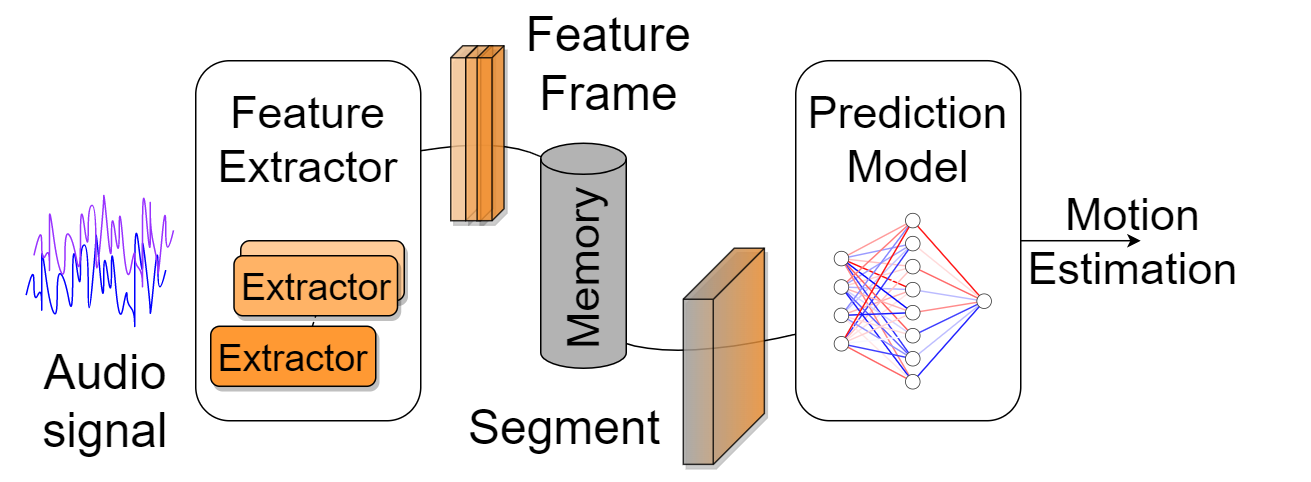
\includegraphics[width=\linewidth]{content/system.drawio.png}
    \caption{Proposed system}
    \label{fig:system}
\end{figure}

Wheels or tracks still form the basis for robot locomotion, although strides
have been made into exotic forms of legged robots \cite{Sanchez09}. Wheeled
mobile systems are useful for practical applications compared with legged
systems because of the simplicity of the mechanisms and control systems and
efficiency in energy consumption \cite{Masayoshi2006}. However, wheeled
systems' performance depends on the traction between the wheels and the ground.
If there is not enough traction, the wheel will slip and the efficiency will
decrease. Traction is a special concern when the robot is expected to move over
granular non-cohesive loose soil. Which is the case for planetary missions
\cite{Amar2007}, construction site applications, and agricultural robots, among
others.

One of the simplest forms of self-contained localization is wheel odometry,
based on wheel encoders that are mounted on a robot to track the number of
revolutions each wheel has made. The number of revolutions is integrated into a
dynamic model to determine the robot's current position relative to the
starting point \cite{OdometrySurvey}. But it performs poorly in the presence of
wheel slippage, accumulating position error (drift).

Another form of self-contained localization is visual odometry, which operates
by incrementally estimating the pose of the vehicle through examination of the
changes that motion induces on the images of its onboard cameras
\cite{ScaramuzzaTutorial}. Similarly, laser odometry estimates the ego-motion
of a vehicle by scan-matching of consecutive laser scans. Unlike wheel
odometry, both visual odometry and laser odometry, are not affected by wheel
slip. They have their drawbacks: visual odometry suffers from poor illumination
and low textured environments; laser might struggle in degenerated scenes where
planar areas are prevalent; both are sensitive to dynamic environments.

Research that improves the robustness of robot localization can be divided into
two trends: To fuse information from different sensors to overcome their
individual limitations \cite{Valente2019,Vargas2021,Ojeda2006} and to make
better use of the available sensor information using deep learning and other
computationally expensive algorithms \cite{Long2021,DFVO}. Therefore, robot
localization robustness has a price. Whether it is the explicit price of extra
sensors or the implicit cost of extra computational resources.